\documentclass[american,titlepage]{ntnuthesis}

% --- Other packages --- %
    \usepackage{microtype}

% --- Tikz --- %
    \usepackage{pgfplots}
    \pgfplotsset{compat=1.15}
    \usepackage{tikz}
    \usetikzlibrary{graphs}
    \usetikzlibrary{arrows}
    \usepackage{tikz-cd}

% --- Ams theorem definitions --- %
    \usepackage{amsthm}

    % --- Defining theorem env --- % 
    \theoremstyle{plain}
    \newtheorem{thm}{Theorem}[section]
    \newtheorem{lemma}[thm]{Lemma}
    \newtheorem{proposition}[thm]{Proposition}
    \newtheorem{corollary}{Corollary}[thm]

    % --- Defining definition env --- %
    \theoremstyle{definition}
    \newtheorem{definition}[thm]{Definition}

    % --- Defining remark env --- %
    \theoremstyle{remark}
    \newtheorem{remark}[thm]{Remark}
    \newtheorem{construction}[thm]{Construction}
    \newtheorem{observation}[thm]{Observation}
    \newtheorem{example}[thm]{Example}

    % --- Defining proof environment --- %

% --- Macros --- %
    \newcommand{\startset}[1]{\{#1\}}

% --- Front page --- %
    \title{Strongly Homotopy Associative Quasi-isomorphisms}
    \shorttitle{Sha Cat}
    \author{Thomas Wilskow Thorbjørnsen}
    \shortauthor{Thorbjørnsen}
    \date{\today}

% --- Bibliography --- %
    \addbibresource{thesis.bib}

% --- Glossary --- %
    
% From https://www.overleaf.com/learn/latex/Glossaries

\makeglossaries % Prepare for adding glossary entries


\newglossaryentry{latex}
{
        name=latex,
        description={Is a mark up language specially suited for
scientific documents}
}

\newglossaryentry{bibliography}
{
        name=bibliography,
        plural=bibliographies,
        description={A list of the books referred to in a scholarly work,
typically printed as an appendix}
}

\newglossaryentry{maths}
{
    name=mathematics,
    description={Mathematics is what mathematicians do}
}


% --------------------
% ----- Acronyms -----
% --------------------

\newacronym{phd}{PhD}{philosophiae doctor}
\newacronym{CoPCSE}{CoPCSE@NTNU}{Community of Practice in Computer ScienceEducation at NTNU}
\newacronym{gcd}{GCD}{Greatest Common Divisor}
 % add glossary and acronym lists before document

% --- Folder structure --- %
    \usepackage{subfiles} 
    % Allows compilation of each subfile, rather to compile everything at once
    % Subfiles must have this file as option while using the documentclass subfile
    % Loading a subfile is done with \subfile{"path-to-file"}

\begin{document}

    % --- Preface --- %
    \subfile{chapters/preface/preface.tex}

    % --- Structure --- %
    \tableofcontents % This lists each listable section, subsection and subsubsection 
    % \listoffigures % This lists each figure
    % \listoftables % This lists each table
    % \lstlistoflistings % This lists each code snippet

    \printglossary[type=\acronymtype] % Print acronyms
    \printglossary                    % Print glossary

    % --- Chapter 1 --- %
    \chapter{Bar and Cobar Construction}

        \documentclass[../../thesis.tex]{subfiles}

\begin{document}
    \section{Algebras, Coalgebras and Twisting Morphisms}

        In this section we will look at a result of associative algebras over a field $\mathbb{K}$. Given a coassociative conilpotent coalgebra $C$ and an associative algebra $A$, we say that a linear transformation $\alpha: C\rightarrow A$ is twisting if it satisfies the Maurar-Cartan equation:
            \begin{equation*}
                \partial\alpha + \alpha\star\alpha = 0.
            \end{equation*}
        Let $Tw(C,A)$ be the set of twisting morphisms, then considering it as a functor $Tw : CoAlg_{\mathbb{K}}^{op}\times Alg_{\mathbb{K}} \rightarrow Ab$ we want to show that it is represented in both arguments. Moreover, this representation give rise to an adjoint pair of functors, called the Bar and Cobar construction.

            \begin{center}
                \begin{tikzcd}
                    Alg_{\mathbb{K}} \ar[bend left]{r}[pos=0.55]{B} \ar[phantom]{r}{\top} & \substack{Conil \\ CoAlg}_{\mathbb{K}} \ar[bend left]{l}[pos=0.45]{\Omega}
                \end{tikzcd}
            \end{center}

        To obtain this result we need to define a twisting morphism. Thus this section will define algebras, coalgebras and convolution algebras before we state the result of the Bar and Cobar construction.

        \subsection{Algebras}

            In this subsection we will look at associative algebras. We will define unital associative algebras and non-unital associative algebras, which we will call algebras and non-unital algebras respectively. The collection of algebras together with homomorphisms between them form the category $Alg_{\mathbb{K}}$ of algebras. Other types of algebras such as augmented and tensor algebras will be defined as well.

            \begin{definition}[Algebra]
                Let $\mathbb{K}$ be a field. An algebra $A$ over $\mathbb{K}$ is a $\mathbb{K}$-module with structure morphisms called multiplication and unit,
                \begin{align*}
                    (\nabla_A) & : A\otimes_{\mathbb{K}}A \rightarrow A \\
                    \nu_A & : \mathbb{K} \rightarrow A,
                \end{align*}
                satisfying the associativity and identity laws. 
                \begin{align*}
                    (associativity)\quad & (a \nabla_A b) \nabla_A c = a \nabla_A (b \nabla_A c) \\
                    (unitality)\quad & \nu_A(1) \nabla_A a = a = a \nabla_A \nu_A(1)
                \end{align*}
            \end{definition}
            \begin{remark}
                Whenever $A$ does not posess a unit morphism, we will call $A$ a non-unital algebra. Only the associativity law must hold.
            \end{remark}
            Alternatively, instead of using equations, we may represent the laws with commutative diagrams. 
            \begin{center}
                (associativity)\quad
                \begin{tikzcd}
                    A \otimes_{\mathbb{K}} A \otimes_{\mathbb{K}} A \ar[]{r}{(\nabla_A)\otimes id_{\mathbb{K}}} \ar[]{d}[]{id_{\mathbb{K}}\otimes (\nabla_A)} & A \otimes_{\mathbb{K}} A \ar[]{d}{(\nabla_A)} \\
                    A \otimes_{\mathbb{K}} A \ar[]{r}[]{(\nabla_A)} & A
                \end{tikzcd} \\
                (unitality) \quad
                \begin{tikzcd}
                    A \otimes_{\mathbb{K}} \mathbb{K} \ar[]{r}[]{id_A \otimes \nu_A} \ar[]{rd}[below]{\simeq} & A \otimes_{\mathbb{K}} A \ar[]{d}[]{(\nabla_A)} & \mathbb{K} \otimes_{\mathbb{K}} A \ar[]{l}[above]{\nu_A \otimes id_A} \ar[]{ld}[]{\simeq}\\
                    & A
                \end{tikzcd}
            \end{center}
            We may also present the structure of algebras by electric circuits. Such circuits are read from top to bottom, where morphisms are composed by lines. Morphisms in such diagrams may be highlighted with figures, conjunctions or twistings. E.g. The multiplication operator may be represented as a converging fork, and the unit as a source.
            \begin{center}
                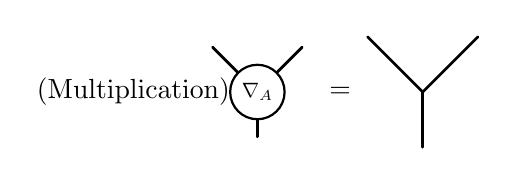
\begin{tikzpicture}[line cap=round,line join=round,>=triangle 45,x=1cm,y=1cm, thick, op/.style={circle, draw, scale = 0.75}, scale = 0.7]
                    \node at (-2.25, 0) {(Multiplication)};
                    
                    \node (1) at (1,1) {};
                    \node (2) at (-1,1) {};
                    \node[op] (3) at (0,0) {$\nabla_A$};
                    \node (4) at (0,-1) {};

                    \graph {
                        (1) --[line width = 1pt] (3);
                        (2) --[line width = 1pt] (3);
                        (3) --[line width = 1pt] (4);
                    };

                    \node at (1.5,0) {$=$};

                    \draw [line width=1pt] (2,1)-- (3,0);
                    \draw [line width=1pt] (3,0)-- (3,-1);
                    \draw [line width=1pt] (4,1)-- (3,0);
                \end{tikzpicture} \quad
                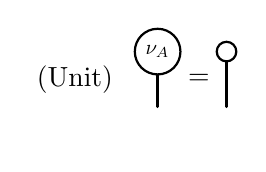
\begin{tikzpicture}[line cap=round,line join=round,>=triangle 45,x=1cm,y=1cm, thick, op/.style={circle, draw, scale=0.75}, scale=0.7]
                    \node at (-1.5,0.5) {(Unit)};
                    
                    \node[op] (1) at (0,1) {$\nu_A$};
                    \draw [line width=1pt] (1) -- (0,0);

                    \node at (0.75, 0.5) {$=$};

                    \node[op, scale=1] (2) at (1.25,1) {};
                    \draw [line width=1pt] (2) -- (1.25,0);

                    \node at (0,-0.5) {};
                \end{tikzpicture}
            \end{center}
            With these operators we obtain the electric laws for an algebra.
            \begin{center}
                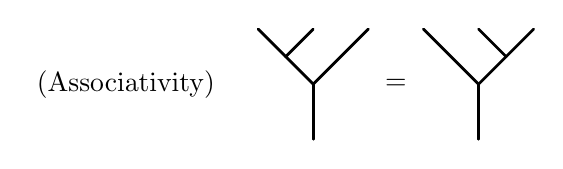
\begin{tikzpicture}[line cap=round,line join=round,>=triangle 45,x=1cm,y=1cm, thick, op/.style={circle, draw, scale=0.75}, scale=0.7]
                    \node at (-2.4,0) {(Associativity)};

                    \draw [line width=1pt] (0,1) -- (1,0);
                    \draw [line width=1pt] (1,0) -- (2,1);
                    \draw [line width=1pt] (0.5,0.5) -- (1,1);
                    \draw [line width=1pt] (1,0) -- (1,-1);

                    \node at (2.5,0) {$=$};

                    \draw [line width=1pt] (3,1) -- (4,0);
                    \draw [line width=1pt] (4,0) -- (5,1);
                    \draw [line width=1pt] (4,1) -- (4.5,0.5);
                    \draw [line width=1pt] (4,0) -- (4,-1);
                \end{tikzpicture} \\

                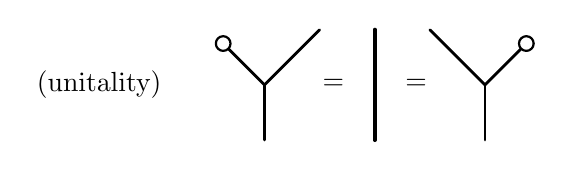
\begin{tikzpicture}[line cap=round,line join=round,>=triangle 45,x=1cm,y=1cm, thick, op/.style={circle, draw, scale=0.75}, scale=0.7]
                    \node at (-2,0) {(unitality)};

                    \node[op, scale=0.75] (1) at (0.25, 0.75) {};
                    \draw [line width=1pt] (1) -- (1,0);
                    \draw [line width=1pt] (1,0) -- (2,1);
                    \draw [line width=1pt] (1,0) -- (1,-1);

                    \node at (2.25,0) {$=$};

                    \draw [line width=1.5pt] (3,1) -- (3,-1);

                    \node at (3.75,0) {$=$};

                    \draw [line width=1pt] (4,1) -- (5,0);
                    \node[op, scale=0.75] (2) at (5.75,0.75) {};
                    \draw [line width=1pt] (5,0) -- (2);
                    \draw [line width=1pt] (5,0) -- (5,-1);
                \end{tikzpicture}
            \end{center}

            \begin{definition}[Algebra homomorphisms]
                Let $A$ and $B$ be algebras. Then $f: A\rightarrow B$ is an algebra homomorphism if
                \begin{enumerate}
                    \item $f$ is $\mathbb{K}$-linear
                    \item $f(ab)=f(a)f(b)$
                    \item $f(\nu_A) = \nu_B$
                \end{enumerate}
                Whenever $A$ and $B$ are non-unital, we only require 1 and 2 for a homomorphism of non-unital algebras.
            \end{definition}

            \begin{definition}[Category of algebras]
                \begin{itemize}
                    \item Let $Alg_{\mathbb{K}}$ denote the category of algebras. It's objects consists of every algebra $A$, and the morphisms are algebra homomorphisms. The sets of morphisms between $A$ and $B$ are denoted as $Alg_{\mathbb{K}}(A,B)$.
                    \item Let $nAlg_{\mathbb{K}}$ denote the category of non-unital algebras. It's objects consists of every non-unital algebra $A$, and the morphisms are non-unital algebra homomorphisms. The sets of morphisms between $A$ and $B$ are denoted as $nAlg_{\mathbb{K}}(A,B)$.
                \end{itemize}
            \end{definition}

            \begin{definition}[Augmented algebras]
                Let $A$ be an algebra. It is called augmented if there is an algebra homomorphism $\varepsilon : A \rightarrow \mathbb{K}$.
            \end{definition}

            If $A$ is an augmented algebra, then it decomposes into $\mathbb{K}\oplus Ker\varepsilon$ as a module. The splitting is given by unitality of the morphism $\varepsilon: A \rightarrow \mathbb{K}$, as we know that $\varepsilon(\nu_A) = id_{\mathbb{K}}$. The kernel of $\varepsilon$ is called the augmentation ideal or redecued algebra and we will denote it as $\bar{A}$. Taking kernels gives an equivalence of categories between augmented algebras and non-unital algebras, with unitization as the quasi-inverse.

            \begin{definition}[Tensor algebra]
                Let $V$ be a $\mathbb{K}$-module. We define the tensor algebra $T(V)$ of $V$ as the module
                \begin{align*}
                    T(V) = \mathbb{K}\oplus V\oplus V^{\otimes 2} \oplus V^{\otimes 3} \oplus ...
                \end{align*}
                Given two strings $v^1..v^i$ and $w^1...w^j$ in $T(V)$ we define the multiplication by the concatenation operation.
                \begin{align*}
                    \nabla_{T(V)} : T(V)\otimes_{\mathbb{K}} T(V) & \rightarrow T(V) \\
                    (v^1...v^i)\otimes(w^1...w^j) & \mapsto v^1...v^iw^1...w^j
                \end{align*}
                The unit is given by including $\mathbb{K}$ into $T(V)$.
                \begin{align*}
                    \nu_{T(V)} : \mathbb{K} & \rightarrow T(V) \\
                    1 & \mapsto 1
                \end{align*}
            \end{definition}

            Observe that the tensor algebra is augmented. The projection from $T(V)$ into $\mathbb{K}$ is an algebra homomorphism, so we may split the tensor algebra into its unit and its augmentation ideal $T(V) \simeq \mathbb{K}\oplus\bar{T(V)}$. We call $\bar{T(V)}$ the reduced tensor algebra.

            \begin{proposition}[Tensor algebra is free]
                The tensor algebra is the free algebra over the category of $\mathbb{K}$-modules, i.e. for any $\mathbb{K}$-module $V$ there is a natural isomorphism $mod_{\mathbb{K}}(V,A)\simeq Alg_{\mathbb{K}}(T(V),A)$.

                The reduced tensor algebra is the fre non-unital algebra over the category of $\mathbb{K}$-modules, i.e. for any $\mathbb{K}$-module $V$ there is a natural isomorphism $mod_{\mathbb{K}}(V,A)\simeq nAlg_{\mathbb{K}}(\bar{T(V)},A)$.
            \end{proposition}

            \begin{proof}
                This proposition should be evident from the description of an algebra homomorphism from a tensor algebra. If $f: T(V) \rightarrow A$ is an algebra homomorphism, then $f$ must satisfy the following conditions:
                \begin{itemize}
                    \item (Unitality)\quad $f(1) = 1$
                    \item (Homomorphism property)\quad Given $v,w\in V$, then $f(vw) = f(v)\nabla_Af(w)$
                \end{itemize}
                By induction, we see that $f$ is completely determined by where it sends the elements of $V$. Thus restriction by the inclusion of $V$ into $T(V)$ induces a bijection.
            \end{proof}

            \begin{definition}[Modules]
                Let $A$ be an algebra. A $\mathbb{K}$-module $M$ is said to be a left (right) $A$-module if there exists a structure morphism $\mu_M : A\otimes_{\mathbb{K}}M \rightarrow A$ ($\mu_M : M\otimes_{\mathbb{K}}A \rightarrow A$) called multiplication. We require that $\mu_M$ is associative with respect to the multiplication and preserves the unit of $A$, i.e. the electric laws are satisfied.
                \begin{center}
                    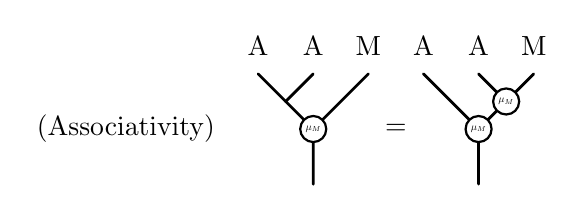
\begin{tikzpicture}[line cap=round,line join=round,>=triangle 45,x=1cm,y=1cm, thick, op/.style={circle, draw, scale=0.75}, scale=0.7]
                        \node at (-2.4,0) {(Associativity)};
                        
                        \node at (0,1.5) {A};
                        \node at (1,1.5) {A};
                        \node at (2,1.5) {M};

                        \node[op, scale = 0.5] (a) at (1,0) {$\mu_M$};

                        \draw [line width=1pt] (0,1) -- (a);
                        \draw [line width=1pt] (a) -- (2,1);
                        \draw [line width=1pt] (0.5,0.5) -- (1,1);
                        \draw [line width=1pt] (a) -- (1,-1);
                        
                        \node at (2.5,0) {$=$};
                        
                        \node at (3,1.5) {A};
                        \node at (4,1.5) {A};
                        \node at (5,1.5) {M};

                        \node[op, scale = 0.5] (b) at (4.5,0.5) {$\mu_M$};
                        \node[op, scale = 0.5] (c) at (4,0) {$\mu_M$};

                        \draw [line width=1pt] (3,1) -- (c);
                        \draw [line width=1pt] (c) -- (b) -- (5,1);
                        \draw [line width=1pt] (4,1) -- (b);
                        \draw [line width=1pt] (c) -- (4,-1);
                    \end{tikzpicture}\\

                    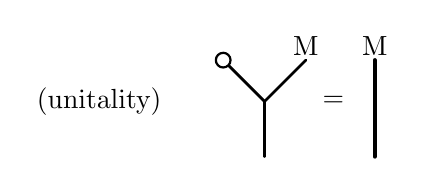
\begin{tikzpicture}[line cap=round,line join=round,>=triangle 45,x=1cm,y=1cm, thick, op/.style={circle, draw, scale=0.75}, scale=0.7]
                        \node at (-2,0) {(unitality)};
    
                        \node at (1.75,1) {M};

                        \node[op, scale=0.75] (1) at (0.25, 0.75) {};
                        \draw [line width=1pt] (1) -- (1,0);
                        \draw [line width=1pt] (1,0) -- (1.75,0.75);
                        \draw [line width=1pt] (1,0) -- (1,-1);
    
                        \node at (2.25,0) {$=$};
    
                        \node at (3,1) {M};

                        \draw [line width=1.5pt] (3,0.75) -- (3,-1);
                    \end{tikzpicture}
                \end{center}
            \end{definition}

            \begin{definition}[A-linear homomorphisms]
                Let $M,N$ be two left $A$-modules. A morphism $f:M\rightarrow N$ is called $A$-linear if it is $\mathbb{K}$-linear and for any $a$ in $A$, $f(am) = af(m)$.
            \end{definition}

            The category of left $A$-modules is denoted as $Mod_A$, where the morphisms are $A$-linear. Likewise, the category of right $A$-modules is denoted as $Mod^A$. 

            \begin{proposition}
                Let $M$ be a $\mathbb{K}$-module. The module $A\otimes_{\mathbb{K}}M$ is a left $A$-module. Moreover, it is the free left module over $\mathbb{K}$-modules, i.e. there is an isomorphism $Mod_{\mathbb{K}}(M,N)\simeq Mod_{A}(A\otimes_{\mathbb{K}}M,N)$.
            \end{proposition}
            
        \subsection{Coalgebras}
            This subsection aims to dualize the definitions from last section. To this end we will define counital coassociative coalgebras and non-counital coassociative coalgebras, which will be called coalgebras and non-counital coalgebras respectively. The collection of coalgebras together with coalgebra homomorphisms is the category $CoAlg_{\mathbb{K}}$. Due to some ill-behavior, this dualization is only a true dualization under some finiteness conditions for the algebras. Thus we will see that the proper dual concept will be of conilpotent coalgebras. We will see that the cofree coalgebra is conilpotent.

            \begin{definition}[Coalgebra]
                Let $\mathbb{K}$ be a field. A coalgebra $C$ over $\mathbb{K}$ is a $\mathbb{K}$-module with structure morphisms called comultiplication and counit,
                \begin{align*}
                    (\Delta_C) & : C \rightarrow C\otimes_{\mathbb{K}}C \\
                    \varepsilon_C & : C \rightarrow \mathbb{K},
                \end{align*}
                satisfying the coassociativity and coidentity laws. 
                \begin{align*}
                    (coassociativity)\quad & (\Delta_C\otimes id_C)\circ\Delta_C(c) = (id_C\otimes\Delta_C)\circ\Delta_C(c) \\
                    (counitality) \quad & (id_C\otimes\varepsilon_C)\circ\Delta_C(c) = c = (\varepsilon_C\otimes id_C)\circ\Delta_C(c)
                \end{align*}
            \end{definition}

            We define repeated application of comultiplication as $\Delta_C^n = (\Delta_C\otimes id_C\otimes ...)\circ\Delta_C^{n-1}$. Notice that the choice of where we put comultiplication in the tensor does not matter, as coassociativity require all of the choices to be equal.

            We may dualize the electric circuits of an algebra to coalgebras. In this manner our structure morphisms would be upside down relative to the algebra morphisms. Thus comultiplication becomes a diverging fork and counit is a sink. 
            \begin{center}
                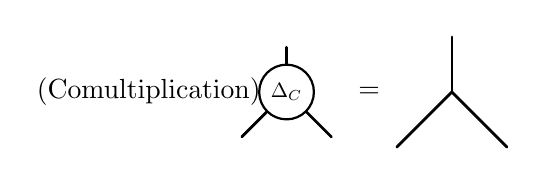
\begin{tikzpicture}[line cap=round,line join=round,>=triangle 45,x=1cm,y=1cm, thick, op/.style={circle, draw, scale = 0.75}, scale = 0.7]
                    \node at (-2.5, 0) {(Comultiplication)};
                    
                    \node (1) at (0,1) {};
                    \node (2) at (-1,-1) {};
                    \node[op] (3) at (0,0) {$\Delta_C$};
                    \node (4) at (1,-1) {};

                    \graph {
                        (1) --[line width = 1pt] (3);
                        (2) --[line width = 1pt] (3);
                        (3) --[line width = 1pt] (4);
                    };

                    \node at (1.5,0) {$=$};

                    \draw [line width=1pt] (2,-1)-- (3,0);
                    \draw [line width=1pt] (3,0)-- (3,1);
                    \draw [line width=1pt] (4,-1)-- (3,0);
                \end{tikzpicture} \quad
                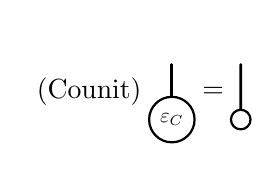
\begin{tikzpicture}[line cap=round,line join=round,>=triangle 45,x=1cm,y=1cm, thick, op/.style={circle, draw, scale=0.75}, scale=0.7]
                    \node at (-1.5,-0.5) {(Counit)};
                    
                    \node[op] (1) at (0,-1) {$\varepsilon_C$};
                    \draw [line width=1pt] (1) -- (0,0);

                    \node at (0.75, -0.5) {$=$};

                    \node[op, scale=1] (2) at (1.25,-1) {};
                    \draw [line width=1pt] (2) -- (1.25,0);

                    \node at (0,0.5) {};
                \end{tikzpicture}
            \end{center}
            We then obtain the electric laws for a coalgebra by flipping the diagrams around.
            \begin{center}
                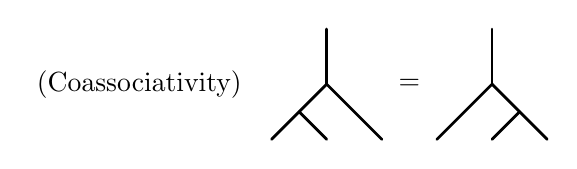
\begin{tikzpicture}[line cap=round,line join=round,>=triangle 45,x=1cm,y=1cm, thick, op/.style={circle, draw, scale=0.75}, scale=0.7]
                    \node at (-2.4,0) {(Coassociativity)};

                    \draw [line width=1pt] (0,-1) -- (1,0);
                    \draw [line width=1pt] (1,0) -- (2,-1);
                    \draw [line width=1pt] (0.5,-0.5) -- (1,-1);
                    \draw [line width=1pt] (1,0) -- (1,1);

                    \node at (2.5,0) {$=$};

                    \draw [line width=1pt] (3,-1) -- (4,0);
                    \draw [line width=1pt] (4,0) -- (5,-1);
                    \draw [line width=1pt] (4,-1) -- (4.5,-0.5);
                    \draw [line width=1pt] (4,0) -- (4,1);
                \end{tikzpicture} \\

                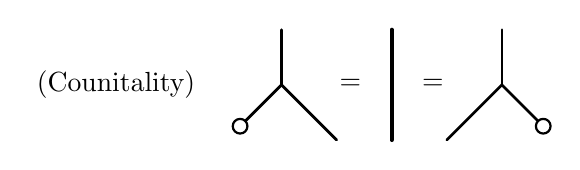
\begin{tikzpicture}[line cap=round,line join=round,>=triangle 45,x=1cm,y=1cm, thick, op/.style={circle, draw, scale=0.75}, scale=0.7]
                    \node at (-2,0) {(Counitality)};

                    \node[op, scale=0.75] (1) at (0.25, -0.75) {};
                    \draw [line width=1pt] (1) -- (1,0);
                    \draw [line width=1pt] (1,0) -- (2,-1);
                    \draw [line width=1pt] (1,0) -- (1,1);

                    \node at (2.25,0) {$=$};

                    \draw [line width=1.5pt] (3,1) -- (3,-1);

                    \node at (3.75,0) {$=$};

                    \draw [line width=1pt] (4,-1) -- (5,0);
                    \node[op, scale=0.75] (2) at (5.75,-0.75) {};
                    \draw [line width=1pt] (5,0) -- (2);
                    \draw [line width=1pt] (5,0) -- (5,1);
                \end{tikzpicture}
            \end{center}

            \begin{definition}[Coalgebra homomorphism]
                Let $C$ and $D$ be coalgebras. Then $f:C\rightarrow D$ is a coalgebra morphism if
                \begin{enumerate}
                    \item $f$ is $\mathbb{K}$-linear
                    \item $(f\otimes f)\circ\Delta_C(c) = \Delta_D(f(c))$
                    \item $\varepsilon_D(f) = \varepsilon_C$
                \end{enumerate}
                Whenever $C$ and $D$ are non-counital, we only require 1 and 2 for a homomorphism of non-counital coalgebras.
            \end{definition}

            \begin{definition}[Category of Coalgebras]
                \begin{itemize}
                    \item Let $CoAlg_{\mathbb{K}}$ denote the category of coalgebras. It's objects consists of every coalgebra $C$, and the morphisms are coalgebra homomorphisms. The sets of morphisms between $C$ and $D$ are denoted as $CoAlg_{\mathbb{K}}(C,D)$.
                    \item Let $nCoAlg_{\mathbb{K}}$ denote the category of non-unital algebras. It's objects consists of every non-unital algebra $C$, and the morphisms are non-unital algebra homomorphisms. The sets of morphisms between $C$ and $D$ are denoted as $nCoAlg_{\mathbb{K}}(C,D)$.
                \end{itemize}
            \end{definition}

            \begin{example}[The coalgebra $\mathbb{K}$]
                The field $\mathbb{K}$ can be given a coalgebra structure over itself. Since $\{1\}$ is a basis for $\mathbb{K}$ we define the structure morphisms as
                \begin{align*}
                    \Delta_{\mathbb{K}}(1) & = 1\otimes 1 \\
                    \varepsilon(1) & = 1.
                \end{align*}
                One may check that these morphisms are indeed coassociative and counital. Thus we may regard our field as either an algebra or coalgebra over itself.
            \end{example}

            \begin{definition}[Coaugmented coalgebras]
                Let $C$ be a coalgebra. $C$ is coagumented if there is a coalgebra homomorphism $\nu:\mathbb{K}\rightarrow C$.
            \end{definition}

            If $C$ is a coaugmented coalgebra, then it splits as $C\simeq \mathbb{K}\oplus Cok\nu$. The splitting is given by counitality of $\nu$, as $\varepsilon_C(\nu) = id_{\mathbb{K}}$. We call the cokernel $Cok\nu = \bar{C}$ for the coaugmentation quotient or reduced coalgebra, and its reduced coproduct may be explicitly given as
            \begin{align*}
                \bar{\Delta}_C(c) = \Delta_C(c) - 1\otimes c - c\otimes 1. 
            \end{align*}

            \begin{definition}[Tensor Coalgebras]
                Let $V$ be a $\mathbb{K}$-module. We define the tensor coalgebra $T^c(V)$ of $V$ as the module
                \begin{align*}
                    T^c(V) = \mathbb{K}\oplus V\oplus V^{\otimes 2}\oplus V^{\otimes 3}\oplus ...
                \end{align*}
                Given a string $v^1...v^i$ in $T(V)$ we define the comultiplication by the deconcatenation operation.
                \begin{align*}
                    \Delta_{T^c(V)}:T^c(V) & \rightarrow T^c(V)\otimes_{\mathbb{K}}T^c(V) \\
                    v^1...v^i & \mapsto 1\otimes(v^1...v^i) + (\sum_{j=1}^{n-1} (v^1...v^{j})\otimes(v^{j+1}...v^i)) + (v^1...v^i)\otimes 1
                \end{align*}
                The counit is given by projecting $T^c(V)$ onto $\mathbb{K}$.
                \begin{align*}
                    \varepsilon_{T^c(V)} : T^c(V) & \rightarrow \mathbb{K} \\
                    1 & \mapsto 1 \\
                    v^1...v^i & \mapsto 0
                \end{align*}
            \end{definition}

            Notice that the tensor coalgebra is coaugmented. Its coaugmentation is given by the inclusion of $\mathbb{K}$ into $T^c(V)$. We may split $T^c(V) \simeq \mathbb{K}\oplus \bar{T^c}(V)$, where $\bar{T^c}(V)$ is the reduced tensor coalgebra.

            In order to get cofreeness for the tensor coalgebra we need some finiteness conditions. This is one of the properties which is ill-behaved when we are dualizing the tensor algebra. The extra assumption which we will need is to assume that the coalgebras are conilpotent. Let $C \simeq \mathbb{K} \oplus \bar{C}$ be a coaugmented coalgebra, we define the coradical filtration of $C$ as a filtration $Fr_0C \subseteq Fr_1C \subseteq ... \subseteq Fr_rC \subseteq ...$ by the submodules:
            \begin{align*}
                Fr_0C & = \mathbb{K} \\
                Fr_rC & = \mathbb{K} \oplus \{c\in\bar{C}\mid \forall n\geq r \bar{\Delta}_C(c) = 0\}.
            \end{align*}

            \begin{definition}[Conilpotent coalgebras]
                Let $C$ be a coaugmented coalgebra. We say that $C$ is conilpotent if its coradical filtration is exhaustive, i.e. $\substack{\varinjlim \\ r}Fr_rC \simeq C$. The subcategory of conilpotent coalgebras will be denoted as $CoAlg^{Conil}_{\mathbb{K}}$.
            \end{proposition}
            \end{definition}

            \begin{proposition}[Conilpotent tensor coalgebra]
                Let $V$ be a $\mathbb{K}$-module. The tensor coalgebra $T^c(V)$ is conilpotent.

            \begin{proof}
                Let $v\in V$, then $\Delta_{T^c(V)}(v)=1\otimes v + v\otimes 1$ and $\bar{\Delta}_{T^c(V)}(v)=0$. We then observe the following:
                \begin{align*}
                    Fr_0T^c(V) & = \mathbb{K} \\
                    Fr_1T^c(V) & = \mathbb{K} \oplus V \\
                    Fr_rT^c(V) & = \bigoplus_{i\leq r} V^{\otimes i}
                \end{align*}
                This shows that the coradical filtration is exhaustive.
            \end{proof}

            \begin{proposition}[Cofree tensor coalgebra]
                The tensor coalgebra is the cofree conilpotent coalgebra over the category of $\mathbb{K}$-modules, i.e. for any $\mathbb{K}$-module $V$ and any conilpotent coalgebra $C$ there is a natural isomorphism $Mod_{\mathbb{K}}(\bar{C}, V)\simeq CoAlg^{Conil}_{\mathbb{K}}(C, T^c(V))$.
            \end{proposition}

            \begin{proof}
                This proposition should be evident from the description of a coalgebra homomorphism into the a tensor coalgebra. If $g:C\rightarrow T^c(V)$ is a coalgebra homomorphism, then $g$ must satisfy the following conditions:
                \begin{enumerate}
                    \item (Coaugmentation)\quad $g(1)=1$
                    \item (Counitality)\quad Given $c\in \bar{C}$ then $\varepsilon_{T^c(V)}\circ g(c)=0$
                    \item (Homomorphism property)\quad Given $c\in C$ then $\Delta_{T^c(V)}(g(c))=(g\otimes g)\circ\Delta_C(c)$
                \end{enumerate}

                We will construct the maps for the isomorphism explicitly. If $g:C\rightarrow T^c(V)$ is a coalgebra homomorphism, then composing with projection gives a map $\pi\circ g:C\rightarrow V$. Note that $\pi\circ g(1)=0$, so this is essentially a map $\pi\circ g:\bar{C}\rightarrow V$. For the other direction, let $\bar{g}:\bar{C}\rightarrow V$. Then we define $g$ as
                \begin{align*}
                    g = id_{\mathbb{K}} \oplus \sum_{i=1}^{\infty}(\otimes^{i}\bar{g})\bar{\Delta}_C^{i-1}.
                \end{align*}
                Observe that $g$ is well defined, since convergence of the sum follows from conilpotency of $C$. One may then check that $g$ is a coalgebra homomorphism, which yields the result.
            \end{proof}

            \begin{definition}[Comodules]
                Let $C$ be a coalgebra. A $\mathbb{K}$-module $M$ is said to ba left (right) $C$-comodule if there exist a structure morphism $\omega_M: M \rightarrow C\otimes_{\mathbb{K}}M$ ($\omega_M: M \rightarrow M\otimes_{\mathbb{K}}C$) called comultiplication. We require that $\omega_M$ is coassociative with respect to the comultiplication of $C$ and preserves the counit of $C$, i.e. the electric laws are satisfied.
                \begin{center}
                    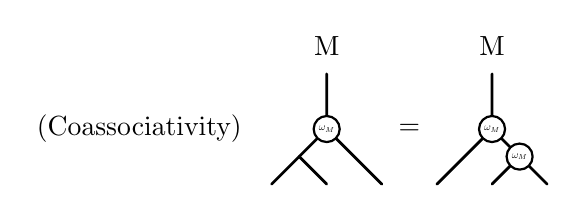
\begin{tikzpicture}[line cap=round,line join=round,>=triangle 45,x=1cm,y=1cm, thick, op/.style={circle, draw, scale=0.75}, scale=0.7]
                        \node at (-2.4,0) {(Coassociativity)};
                        
                        \node at (1,1.5) {M};

                        \node[op, scale = 0.5] (a) at (1,0) {$\omega_M$};

                        \draw [line width=1pt] (0,-1) -- (a);
                        \draw [line width=1pt] (a) -- (2,-1);
                        \draw [line width=1pt] (0.5,-0.5) -- (1,-1);
                        \draw [line width=1pt] (a) -- (1,1);
                        
                        \node at (2.5,0) {$=$};
                        
                        \node at (4,1.5) {M};

                        \node[op, scale = 0.5] (b) at (4.5,-0.5) {$\omega_M$};
                        \node[op, scale = 0.5] (c) at (4,0) {$\omega_M$};

                        \draw [line width=1pt] (3,-1) -- (c);
                        \draw [line width=1pt] (c) -- (b) -- (5,-1);
                        \draw [line width=1pt] (4,-1) -- (b);
                        \draw [line width=1pt] (c) -- (4,1);
                    \end{tikzpicture}\\

                    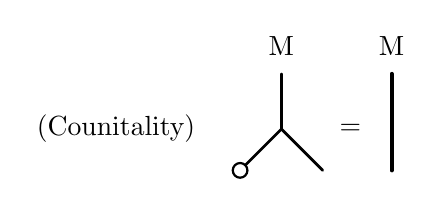
\begin{tikzpicture}[line cap=round,line join=round,>=triangle 45,x=1cm,y=1cm, thick, op/.style={circle, draw, scale=0.75}, scale=0.7]
                        \node at (-2,0) {(Counitality)};
    
                        \node at (1,1.5) {M};

                        \node[op, scale=0.75] (1) at (0.25, -0.75) {};
                        \draw [line width=1pt] (1) -- (1,0);
                        \draw [line width=1pt] (1,0) -- (1.75,-0.75);
                        \draw [line width=1pt] (1,0) -- (1,1);
    
                        \node at (2.25,0) {$=$};
    
                        \node at (3,1.5) {M};

                        \draw [line width=1.5pt] (3,-0.75) -- (3,1);
                    \end{tikzpicture}
                \end{center}
            \end{definition}

            \begin{definition}[C-colinear homomorphism]
                Let $M,N$ be two left $C$-comodules. A morphism $g:M\rightarrow N$ is called $C$-colinear if it is $\mathbb{K}$-linear and for any $m$ in $M$, $\omega_N(g(m)) = (id_C\otimes g)\omega_M(m)$.
            \end{definition}

            The category of left $C$-comodules is denoted as $CoMod_C$, where the morphisms are $C$-colinear. Likewise, the category of right $C$-comodules is denoted as $CoMod^C$.

            \begin{proposition}
                Let $M$ be a $\mathbb{K}$-module. The module $C\otimes_{\mathbb{K}}M$ is a left $C$-comodule. Moreover, it is the cofree left comodule over $\mathbb{K}$-modules, i.e. there is an isomorphism $Mod_{\mathbb{K}}(N,M)\simeq CoMod_C(N,C\otimes_{\mathbb{K}}M)$. 
            \end{proposition}

        \subsection{Derivations, Coderivations and Convolution Algebras}

        \subsection{Twisting Morphisms}


    \section{Strongly Homotopy Associative Algebras, Coalgebras and Twisting Morphisms}

        \subsection{Sha Algebras}

        \subsection{Sha Coalgebras}

        \subsection{Twisting Sha Morphisms}
\end{document}

    \chapter*{\bibname}
    \printbibliography[heading=none]

    % % First paper

\begin{paper}{papers/landes1951scrutiny.pdf}{paper:scrutiny}
    Here, you may add a description of the paper, an illustration, or just give the bibliographic reference:
    \begin{quote}
        \fullcite{landes1951scrutiny}
    \end{quote}
    Or you may leave it empty, if you like.
\end{paper}

% Second paper etc.

    % --- Appendix A --- %

    \appendix
% \chapter{Additional Material}
\label{app:additional}

Additional material that does not fit in the main thesis but may still be relevant to share, e.g., raw data from experiments and surveys, code listings, additional plots, pre-project reports, project agreements, contracts, logs etc., can be put in appendices. Simply issue the command \texttt{\textbackslash appendix} in the main \texttt{.tex} file, and make one chapter per appendix.

If the appendix is in the form of a ready-made PDF file, it should be supported by a small descriptive text, and included using the \texttt{pdfpages} package. To illustrate how it works, a standard project agreement (for the IE faculty at NTNU in Gjøvik) is attached here. You would probably want the included PDF file to begin on an odd (right hand) page, which is achieved by using the \texttt{\textbackslash cleardoublepage} command immediately before the \texttt{\textbackslash includepdf[]\{\}} command. Use the option \texttt{[pages=-]} to include all pages of the PDF document, or, e.g., \texttt{[pages=2-4]} to include only the given page range.

\cleardoublepage
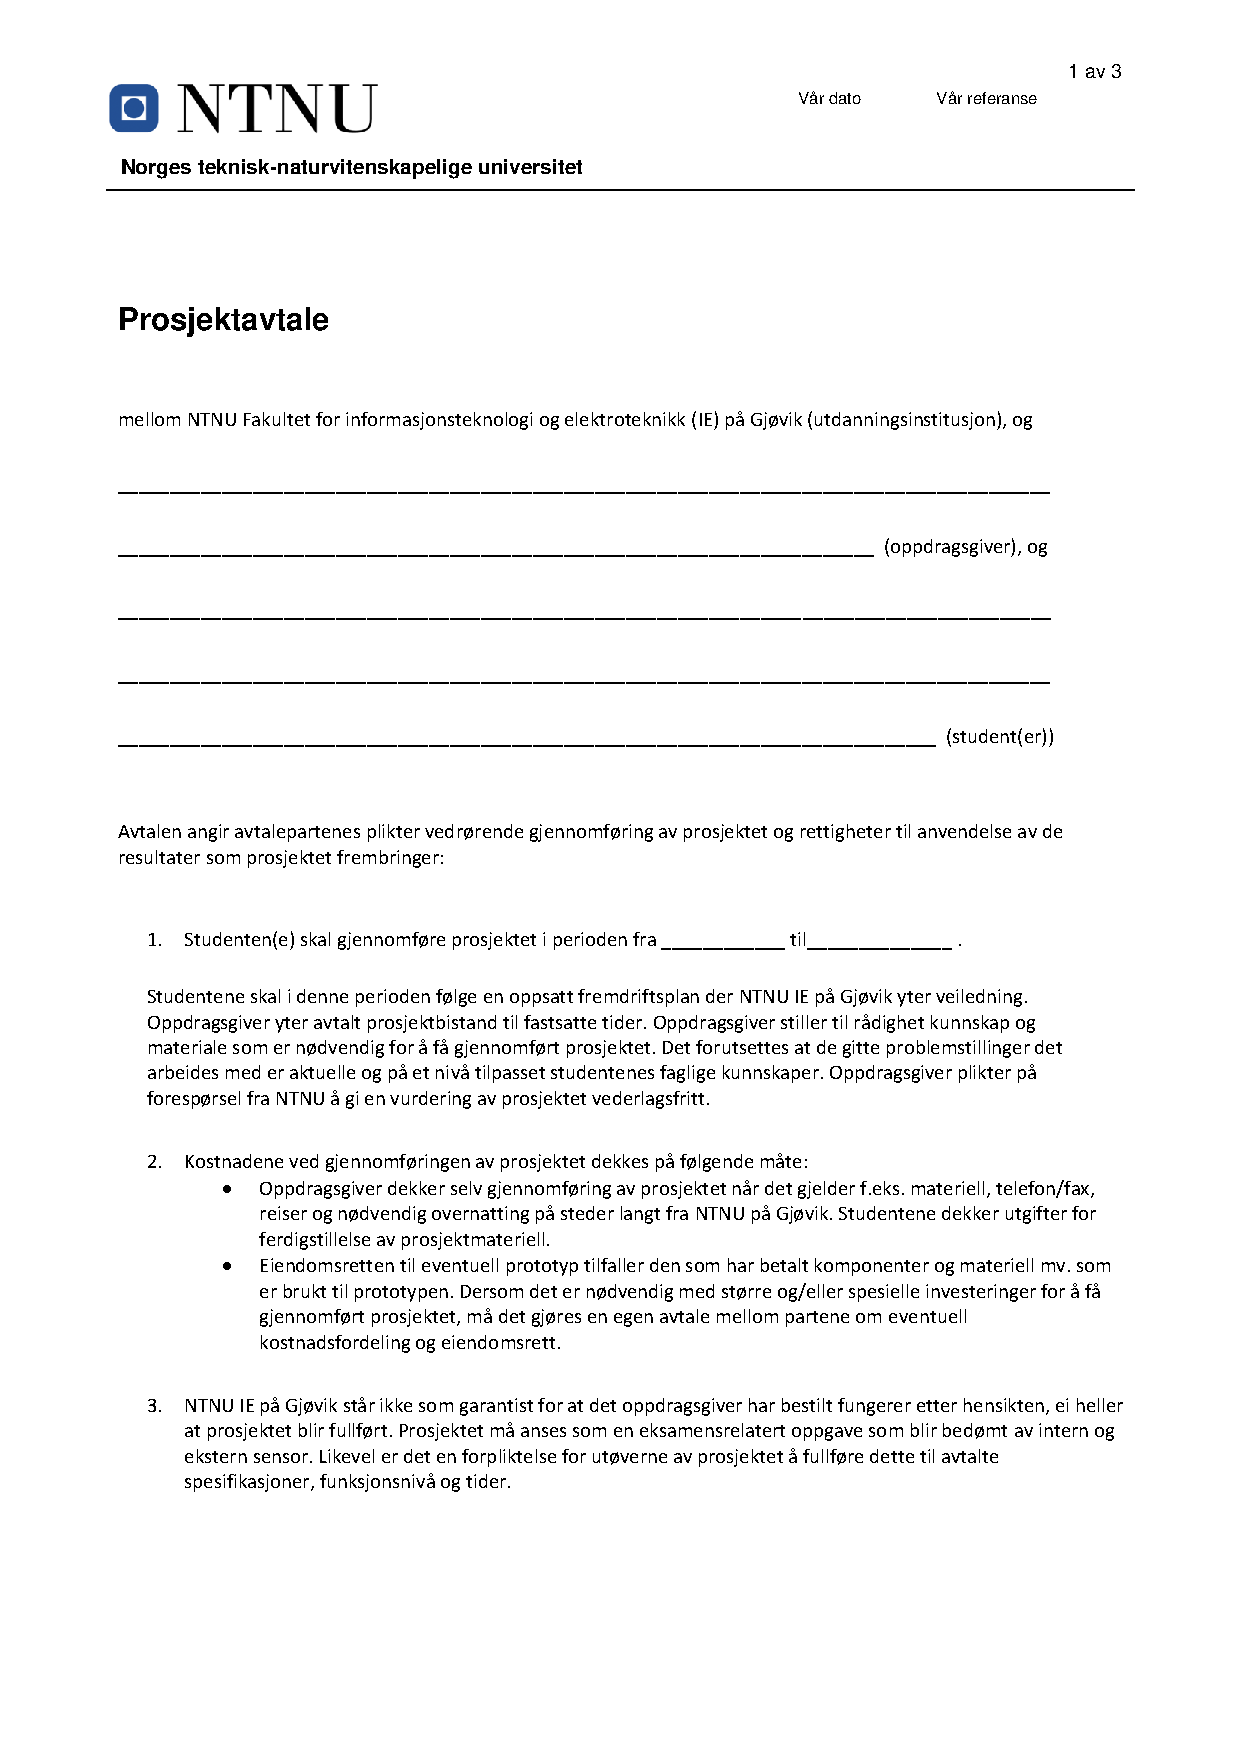
\includepdf[pages=-]{appendices/NTNUProsjektavtale.pdf}

\end{document}
